\documentclass[11pt,a4paper,oneside]{report}

\newcommand{\DocumentTitle}{System Design and Implementation Report}
\newcommand{\DocumentSummary}{This report documents the implemented Mini Payment Gateway as an academic project artifact. It covers requirements, architecture, database design, user interface design, implementation structure, API design, and testing evidence while staying aligned with the behavior currently present in the repository.}

\providecommand{\ProjectTitle}{Mini Payment Gateway}
\providecommand{\CourseName}{Introduction to Software Engineering}
\providecommand{\GroupName}{Group 15}
\providecommand{\AuthorList}{Le Nguyen Phuoc Thanh, Hoang Van Nhan, Ngo Minh Quang, Vu Tran An Khanh, Do Hoang Nam Khanh}
\providecommand{\InstitutionName}{Hanoi University of Science and Technology}
\providecommand{\SubmissionDate}{\today}
\providecommand{\DocumentTitle}{Project Document}
\providecommand{\DocumentSummary}{This document describes the implemented behavior of the Mini Payment Gateway project.}

\usepackage[a4paper,margin=1in]{geometry}
\usepackage[T1]{fontenc}
\usepackage[utf8]{inputenc}
\usepackage{lmodern}
\usepackage{graphicx}
\usepackage{xcolor}
\usepackage{hyperref}
\usepackage{booktabs}
\usepackage{tabularx}
\usepackage{longtable}
\usepackage{array}
\usepackage{enumitem}
\usepackage{float}
\usepackage{caption}
\usepackage{subcaption}
\usepackage{listings}
\usepackage{tikz}
\usepackage{pdflscape}

\usetikzlibrary{arrows.meta,positioning,fit,shapes.geometric}
\graphicspath{{figures/}}

\definecolor{mpgNavy}{HTML}{0E2A36}
\definecolor{mpgTeal}{HTML}{0B797C}
\definecolor{mpgMint}{HTML}{DDF3EA}
\definecolor{mpgWarn}{HTML}{C8892E}
\definecolor{mpgDanger}{HTML}{B54B42}
\definecolor{mpgPaper}{HTML}{F7F8FA}
\definecolor{mpgInk}{HTML}{17202A}
\definecolor{mpgMuted}{HTML}{4E5D78}
\definecolor{codeBg}{HTML}{F4F6F8}

\hypersetup{
  colorlinks=true,
  linkcolor=mpgTeal,
  urlcolor=mpgTeal,
  citecolor=mpgTeal,
  pdftitle={\ProjectTitle: \DocumentTitle},
  pdfauthor={\AuthorList}
}

\setlist[itemize]{leftmargin=1.5em,itemsep=0.2em,topsep=0.2em}
\setlist[enumerate]{leftmargin=1.7em,itemsep=0.2em,topsep=0.2em}
\renewcommand{\arraystretch}{1.18}
\setlength{\parskip}{0.45em}
\setlength{\parindent}{0pt}
\setcounter{tocdepth}{2}
\setcounter{secnumdepth}{2}

\captionsetup{
  font=small,
  labelfont=bf
}

\newcolumntype{Y}{>{\raggedright\arraybackslash}X}
\newcolumntype{L}[1]{>{\raggedright\arraybackslash}p{#1}}
\newcommand{\bodyrowrule}{\specialrule{0.3pt}{0.12em}{0.12em}}
\newcommand{\docbox}[2]{%
  \begingroup
  \setlength{\fboxsep}{8pt}%
  \noindent\fcolorbox{mpgTeal!65}{mpgMint}{%
    \begin{minipage}{0.95\linewidth}
      \textbf{#1}\par
      #2
    \end{minipage}%
  }%
  \endgroup
}
\newcommand{\restrictedbox}[1]{\docbox{Restricted / Internal Use}{#1}}

\lstdefinestyle{mpglisting}{
  backgroundcolor=\color{codeBg},
  basicstyle=\ttfamily\small,
  breaklines=true,
  columns=fullflexible,
  frame=single,
  rulecolor=\color{mpgMuted!35},
  framerule=0.4pt,
  xleftmargin=0.4em,
  xrightmargin=0.4em,
  aboveskip=0.8em,
  belowskip=0.8em
}
\lstdefinelanguage{json}{
  basicstyle=\ttfamily\small,
  showstringspaces=false,
  breaklines=true,
  morestring=[b]",
  stringstyle=\color{mpgTeal},
  morecomment=[l]{//},
  commentstyle=\color{mpgMuted},
  morekeywords={true,false,null}
}
\lstset{style=mpglisting}

\tikzset{
  box/.style={
    draw=mpgNavy!35,
    rounded corners=3pt,
    fill=mpgPaper,
    align=center,
    minimum height=10mm,
    inner sep=5pt,
    font=\small
  },
  actor/.style={
    draw=mpgTeal!55,
    rounded corners=3pt,
    fill=mpgMint,
    align=center,
    minimum height=10mm,
    inner sep=5pt,
    font=\small
  },
  boundary/.style={
    draw=mpgNavy!45,
    dashed,
    rounded corners=5pt,
    inner sep=7pt
  },
  db/.style={
    cylinder,
    shape border rotate=90,
    aspect=0.22,
    draw=mpgNavy!45,
    fill=mpgPaper,
    align=center,
    minimum height=14mm,
    minimum width=24mm,
    font=\small
  },
  arrow/.style={-{Latex[length=2.2mm]}, thick, draw=mpgNavy!75},
  autharrow/.style={-{Latex[length=2.2mm]}, thick, draw=mpgTeal}
}

\newcommand{\safeimage}[3][0.92\linewidth]{%
  \IfFileExists{figures/#2}{%
    \includegraphics[width=#1]{figures/#2}%
  }{%
    \fbox{%
      \begin{minipage}[c][0.24\textheight][c]{#1}
        \centering
        \vspace{0.5em}
        \textbf{Screenshot placeholder}\\[0.4em]
        \texttt{figures/#2}\\[0.4em]
        #3
      \end{minipage}
    }%
  }%
}

\newcommand{\apiendpoint}[2]{\texttt{#1 #2}}
\newcommand{\routecell}[1]{\begin{minipage}[t]{\linewidth}\raggedright #1\end{minipage}}
\newcommand{\apiid}[1]{\texttt{#1}}
\newcommand{\code}[1]{\nolinkurl{#1}}
\newcommand{\apiblockheading}[1]{%
  \par\addvspace{0.85em}%
  \noindent\textbf{#1}\par\smallskip%
}
\newcommand{\frontchapter}[1]{%
  \ifcsname chapter\endcsname
    \chapter*{#1}\addcontentsline{toc}{chapter}{#1}%
  \else
    \section*{#1}\addcontentsline{toc}{section}{#1}%
  \fi
}


\begin{document}

\hypersetup{pageanchor=false}
\makempgtitlepage
\clearpage
\hypersetup{pageanchor=true}

\pagenumbering{roman}

\frontchapter{Abstract}
The Mini Payment Gateway is an implemented MVP payment gateway for merchant
onboarding, dynamic QR payment creation, provider result callbacks, full
refunds, webhook delivery, operational investigation, and dashboard-based
merchant visibility. The system combines a FastAPI backend, PostgreSQL
database, an internal Ops Dashboard, and a separate Merchant Dashboard.

The report is intentionally implementation-faithful. It focuses on the current
repository state rather than speculative features, and it uses the companion
API document in \code{api-documentation.tex} for the detailed endpoint
contracts.

\tableofcontents
\listoffigures
\listoftables

\frontchapter{Glossary and Acronyms}
\begin{longtable}{L{0.20\textwidth}L{0.70\textwidth}}
\toprule
\textbf{Term} & \textbf{Meaning} \\
\midrule
\endfirsthead
\toprule
\textbf{Term} & \textbf{Meaning} \\
\midrule
\endhead
API & Application Programming Interface. \\
E2E & End-to-end verification across multiple components. \\
HMAC & Hash-based message authentication code used by merchant-facing APIs. \\
MVP & Minimum viable product scope implemented for the project. \\
Ops & Internal operations role used for day-to-day support workflows. \\
RBAC & Role-based access control for internal and merchant-facing session users. \\
QR & Quick response payment payload returned to merchants during payment creation. \\
\bottomrule
\end{longtable}

\clearpage
\pagenumbering{arabic}

\chapter{System Requirements and Problem Analysis}

The Mini Payment Gateway is positioned as an implemented MVP rather than a full
payment platform. Its purpose is to support merchant onboarding, QR-based
payment creation, asynchronous provider result processing, full refunds,
webhook delivery, operational investigation, and merchant self-visibility
through a separate dashboard experience.

\section{Problem Context}

The gateway solves two connected problems. First, merchants need a small but
reliable payment interface for creating QR payments, receiving asynchronous
provider outcomes, querying transaction status, and requesting full refunds.
Second, internal operators need visibility and recovery tools because payment
systems are asynchronous by nature: callbacks can arrive late, webhook delivery
can fail, and merchant readiness must be enforced before money-flow APIs are
usable.

The dashboard work revealed an architectural constraint that strongly shaped the
project. A merchant-facing dashboard cannot safely be implemented as frontend
screens alone. It requires a separate portal authentication model, merchant-
scoped read APIs, a dedicated merchant user table, and internal provisioning
flows. Without these boundaries, the system would either misuse merchant API
credentials for human login or risk cross-merchant data exposure.

\section{Implemented Scope And Non-Goals}

\begin{table}[H]
\centering
\caption{Implemented system scope}
\begin{tabularx}{\textwidth}{L{0.24\textwidth}Y}
\toprule
\textbf{Area} & \textbf{Implemented capability} \\
\midrule
Merchant lifecycle & Create merchants, submit and review onboarding evidence, create or rotate credentials, activate, suspend, and disable merchants. \\
Payments & Create dynamic QR payments, enforce semantic idempotency, query by transaction id or order id, and process provider payment result callbacks. \\
Refunds & Create full refunds, enforce refund rules, query refund state, and process provider refund result callbacks. \\
Webhooks & Create durable signed outbound webhook events, store delivery attempts, apply retry policy, and support internal manual retry. \\
Ops Dashboard & Internal operator interface for auth, RBAC, merchant workflows, evidence inspection, reconciliation, audit, internal users, and portal-user provisioning. \\
Merchant Dashboard & Merchant-scoped read-only interface for overview, analytics, payments, refunds, webhooks, profile, credentials, and password change. \\
Testing & Backend unit, route, and E2E tests; frontend typecheck, test, and build; compose validation; and browser smoke procedures. \\
\bottomrule
\end{tabularx}
\end{table}

The following items are intentionally out of scope for the implemented MVP:

\begin{itemize}
  \item settlement ledger and accounting workflows;
  \item disputes or chargebacks;
  \item partial refunds;
  \item multi-provider routing;
  \item merchant self-service onboarding;
  \item merchant profile editing from the Merchant Dashboard;
  \item production-grade notification, TLS, and observability hardening.
\end{itemize}

\section{Functional Requirements}

\begin{longtable}{L{0.24\textwidth}L{0.30\textwidth}L{0.36\textwidth}}
\caption{Functional requirements}\\
\toprule
\textbf{Requirement group} & \textbf{Rule} & \textbf{Implemented decision} \\
\midrule
\endfirsthead
\toprule
\textbf{Requirement group} & \textbf{Rule} & \textbf{Implemented decision} \\
\midrule
\endhead
Merchant lifecycle & Merchant statuses are \texttt{PENDING\_REVIEW}, \texttt{ACTIVE}, \texttt{REJECTED}, \texttt{SUSPENDED}, and \texttt{DISABLED}. & Onboarding approval is stored on \texttt{merchant\_onboarding\_cases}; operational status remains on \texttt{merchants}. \\
Payment creation & One active payment is allowed per merchant and order. & A \texttt{PENDING} payment is reused only when the duplicate request is semantically identical; success blocks a new attempt. \\
Payment states & Persisted states are \texttt{PENDING}, \texttt{SUCCESS}, \texttt{FAILED}, and \texttt{EXPIRED}. & Provider callbacks finalize pending payments, while late or mismatched evidence is routed to reconciliation. \\
Refunds & Only full refunds are implemented; refund window is seven days from \texttt{paid\_at}. & Refund records use \texttt{REFUND\_PENDING}, \texttt{REFUNDED}, and \texttt{REFUND\_FAILED}. Partial refunds are rejected by design. \\
Webhooks & HTTP 2xx means delivered; retry schedule is 1, 5, and 15 minutes after the first failure. & Delivery attempts are persisted; exhausted events become \texttt{FAILED}; internal Ops can manually retry eligible failed events. \\
Dashboards & Ops and Merchant users require different surfaces. & Ops Dashboard is internal and mutable; Merchant Dashboard is read-only except password change. \\
\bottomrule
\end{longtable}

\section{Technical Requirements}

The backend protects each boundary with the correct authentication mechanism.
Merchant backend integrations use HMAC headers:
\texttt{X-Merchant-Id}, \texttt{X-Access-Key}, \texttt{X-Timestamp}, and
\texttt{X-Signature}. Internal users authenticate through an HttpOnly session
cookie. Merchant portal users authenticate through a separate HttpOnly session
cookie with merchant scope derived from the authenticated portal account.

The system also enforces persistence rules where practical:

\begin{itemize}
  \item one active credential per merchant;
  \item one pending payment per merchant and order;
  \item one logical refund per merchant and refund id;
  \item at most one successful full refund per payment;
  \item positive monetary values and non-negative attempt counters;
  \item merchant-scoped analytics indexes for payment, refund, and webhook
  records.
\end{itemize}

\section{Operational Requirements}

The gateway must remain supportable by internal operators. Every important
manual action carries an audit reason, and audit rows capture the event code,
entity identity, actor type, actor id, before and after snapshots, and
timestamp. Sensitive fields such as raw credential secrets are masked in
responses and audit snapshots.

The merchant-facing dashboard must help merchants inspect their own data without
seeing internal reconciliation workflows, raw credential secrets, or data owned
by other merchants. This requirement directly drives the dedicated merchant
portal authentication model and the rule that Merchant Dashboard APIs never
accept a client-supplied \texttt{merchant\_id} for read scope after login.

\chapter{Use-Case Analysis}

\section{Actor Overview}

\begin{table}[H]
\centering
\caption{Implemented actors}
\begin{tabularx}{\textwidth}{L{0.23\textwidth}Y}
\toprule
\textbf{Actor} & \textbf{Role in the system} \\
\midrule
Admin & Privileged internal user who can manage merchants, internal users, credentials, and merchant portal users. \\
Ops & Day-to-day internal operations user who can inspect operational evidence and execute allowed lifecycle and recovery workflows. \\
Merchant backend & Merchant-owned server application that calls payment and refund APIs using HMAC credentials. \\
Merchant portal user & Human merchant user who logs into Merchant Dashboard using merchant id, email, and password. \\
Provider simulator & Simulated external provider that sends payment and refund result callbacks. \\
Scheduler/worker trigger & External trigger that invokes implemented expiration and due-webhook delivery services. \\
\bottomrule
\end{tabularx}
\end{table}

\section{Core Gateway Use Cases}

\begin{longtable}{L{0.11\textwidth}L{0.24\textwidth}L{0.19\textwidth}L{0.36\textwidth}}
\caption{Core implemented use cases}\\
\toprule
\textbf{ID} & \textbf{Use case} & \textbf{Primary actor} & \textbf{Result} \\
\midrule
\endfirsthead
\toprule
\textbf{ID} & \textbf{Use case} & \textbf{Primary actor} & \textbf{Result} \\
\midrule
\endhead
UC001 & Onboard and activate merchant & Admin/Ops & Merchant profile, onboarding case, credential, activation status, and audit trail are created. \\
UC002 & Create dynamic QR payment & Merchant backend & A pending payment and QR payload are created or an identical pending payment is reused. \\
UC003 & Process payment result callback & Provider simulator & Callback evidence is stored; the pending payment becomes success or failed, or reconciliation evidence is created. \\
UC004 & Create full refund and process result & Merchant backend and provider simulator & A full refund is created and later finalized from provider evidence. \\
UC005 & Deliver webhook with retry and manual recovery & Scheduler/worker trigger, Admin/Ops & Webhook attempts are persisted, retries are scheduled, and failed events can be recovered manually. \\
\bottomrule
\end{longtable}

\section{Dashboard Use Cases}

\begin{longtable}{L{0.12\textwidth}L{0.28\textwidth}L{0.20\textwidth}L{0.30\textwidth}}
\caption{Implemented dashboard use cases}\\
\toprule
\textbf{ID} & \textbf{Use case} & \textbf{Actor} & \textbf{Implemented behavior} \\
\midrule
\endfirsthead
\toprule
\textbf{ID} & \textbf{Use case} & \textbf{Actor} & \textbf{Implemented behavior} \\
\midrule
\endhead
DUC001 & Login and view operations overview & Admin/Ops & Internal users authenticate and inspect operational metrics. \\
DUC002 & Manage merchant lifecycle & Admin/Ops & Users create merchants, inspect onboarding and credentials, and apply allowed lifecycle actions. \\
DUC003 & Provision merchant portal users & Admin & Admin creates, updates, deactivates or reactivates, and resets merchant portal users. \\
DUC004 & Inspect operational evidence & Admin/Ops & Users inspect payments, refunds, webhooks, reconciliation, and audit logs. \\
DUC005 & Login and change password & Merchant portal user & Merchant users authenticate with a portal session and can change their own password. \\
DUC006 & View overview and analytics & Merchant portal user & Users view scoped summary metrics and 7, 30, or 90 day analytics. \\
DUC007 & Explore payments, refunds, and webhooks & Merchant portal user & Users browse and inspect records owned by their merchant only. \\
DUC008 & View profile and credentials & Merchant portal user & Users read merchant profile and credential metadata without raw secrets. \\
\bottomrule
\end{longtable}

\section{Use-Case Diagram}

\begin{figure}[H]
\centering
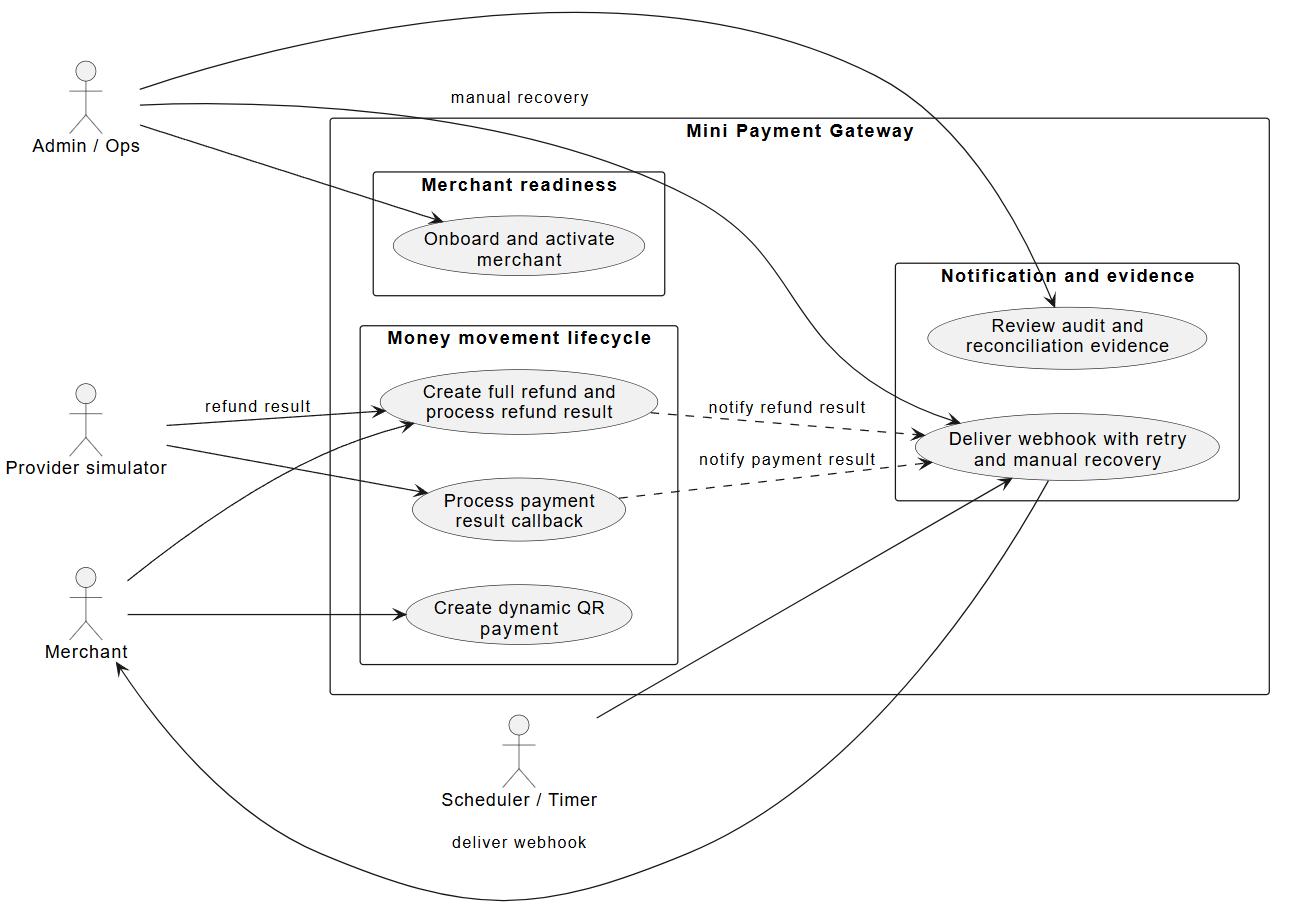
\includegraphics[width=\linewidth]{figures/general-usecase.png}
\caption{Implemented use-case overview. Operational dashboard use cases are
separated from merchant money-flow use cases.}
\end{figure}

\chapter{User Stories}

The user stories are grouped by actor so that the report can connect user
intent to the implemented workflows and boundaries.

\begin{longtable}{L{0.17\textwidth}L{0.37\textwidth}L{0.36\textwidth}}
\caption{Implemented user stories}\\
\toprule
\textbf{ID} & \textbf{Story} & \textbf{Acceptance criteria} \\
\midrule
\endfirsthead
\toprule
\textbf{ID} & \textbf{Story} & \textbf{Acceptance criteria} \\
\midrule
\endhead
US-ADMIN-01 & As an Admin, I want to create and review merchants so that only approved merchants can use the gateway. & Admin can create a merchant, submit and review onboarding evidence, create credentials, and activate the merchant. \\
US-ADMIN-02 & As an Admin, I want to manage internal users so that operations access can be controlled. & Admin can list, create, update, deactivate or reactivate, and reset internal user passwords. \\
US-ADMIN-03 & As an Admin, I want to provision merchant dashboard users so that merchants can inspect their own gateway data. & Admin can create, update, deactivate or reactivate, and reset merchant portal users from merchant detail. \\
US-OPS-01 & As an Ops user, I want to monitor operational queues so that failed or pending work can be handled quickly. & Ops can log in, view metrics and charts, and navigate to payments, refunds, webhooks, and reconciliation. \\
US-OPS-02 & As an Ops user, I want to manage merchant lifecycle states safely. & Ops can perform allowed lifecycle actions with a required reason and audit trail. \\
US-OPS-03 & As an Ops user, I want to inspect webhook attempts so failed notifications can be retried or explained. & Ops can open webhook detail, see attempts, and retry failed webhook events where allowed. \\
US-MERCHANT-01 & As a merchant operator, I want to log in without API credentials. & Merchant user logs in with merchant id, email, and password; the session is separate from HMAC API credentials. \\
US-MERCHANT-02 & As a merchant operator, I want to see overview metrics. & Overview shows summary cards and compact charts for the logged-in merchant only. \\
US-MERCHANT-03 & As a merchant operator, I want interactive analytics with exact values. & Analytics supports 7, 30, and 90 day ranges, tooltips, data tables, and drill-down links. \\
US-MERCHANT-04 & As a merchant operator, I want to inspect payments, refunds, and webhooks for support questions. & Explorer pages list and show detail for only the logged-in merchant's records. \\
US-VIEWER-01 & As a merchant business viewer, I want to view revenue and success-rate trends. & Viewer can open Overview and Analytics, read chart values, and switch date ranges. \\
US-VIEWER-02 & As a merchant business viewer, I want read-only credential metadata. & Credentials page shows access key, secret suffix, status, and timestamps only. \\
\bottomrule
\end{longtable}

\chapter{System Architecture}

\section{System Context}

\begin{figure}[H]
\centering
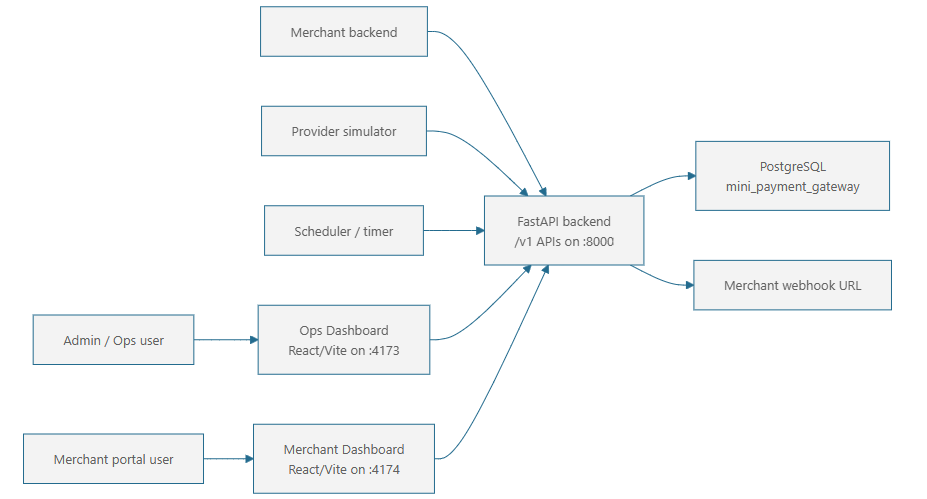
\includegraphics[width=\linewidth]{figures/system-context-diagram.png}
\caption{System context diagram for the implemented Mini Payment Gateway.}
\end{figure}

The implemented system consists of four main runtime components: a FastAPI
backend, PostgreSQL, the internal Ops Dashboard, and the Merchant Dashboard.
The dashboards are not presentation-only shells. Each depends on dedicated API
surfaces, access boundaries, and data representations that match its actor.

\section{Runtime Topology}

\begin{table}[H]
\centering
\caption{Runtime components and responsibilities}
\begin{tabularx}{\textwidth}{L{0.22\textwidth}L{0.24\textwidth}Y}
\toprule
\textbf{Component} & \textbf{Runtime shape} & \textbf{Responsibility} \\
\midrule
FastAPI backend & Application service & Exposes merchant APIs, provider callbacks, internal Ops APIs, internal auth, merchant portal auth, analytics, and recovery endpoints. \\
PostgreSQL & Persistent database & Stores merchant, transaction, refund, webhook, callback, reconciliation, audit, internal user, and merchant user data. \\
Ops Dashboard & Separate frontend application & Supports internal monitoring, merchant operations, user administration, and evidence review. \\
Merchant Dashboard & Separate frontend application & Supports merchant-scoped overview, analytics, explorers, profile, credentials, and password change. \\
\bottomrule
\end{tabularx}
\end{table}

\section{Authentication, Authorization, And Trust Boundaries}

\begin{table}[H]
\centering
\caption{Actor and authentication matrix}
\begin{tabularx}{\textwidth}{L{0.20\textwidth}L{0.21\textwidth}L{0.24\textwidth}Y}
\toprule
\textbf{Actor} & \textbf{API surface} & \textbf{Authentication} & \textbf{Scope source} \\
\midrule
Merchant backend & Merchant API & HMAC headers & Authenticated merchant credential. \\
Admin/Ops user & Ops API & Internal HttpOnly session cookie & Internal user role \texttt{ADMIN} or \texttt{OPS}. \\
Admin user & Ops portal-user API & Internal HttpOnly session cookie & Internal \texttt{ADMIN} role. \\
Merchant portal user & Merchant Portal API & Merchant HttpOnly session cookie & \texttt{merchant\_users.merchant\_db\_id}. \\
Provider simulator & Provider callback API & Environment-local simulator trust in MVP & Callback payload references existing payment or refund rows. \\
\bottomrule
\end{tabularx}
\end{table}

\begin{figure}[H]
\centering
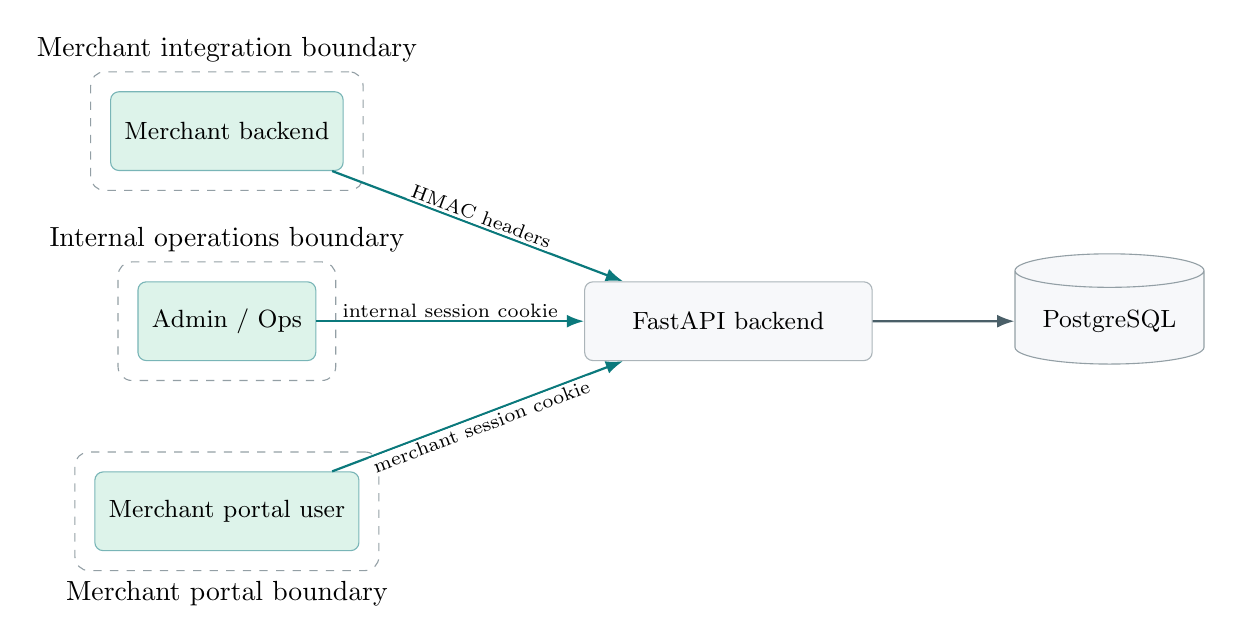
\begin{tikzpicture}[node distance=14mm and 18mm]
  \node[actor] (merchantBackend) {Merchant backend};
  \node[actor, below=of merchantBackend] (opsUser) {Admin / Ops};
  \node[actor, below=of opsUser] (portalUser) {Merchant portal user};
  \node[box, right=34mm of opsUser, text width=33mm] (api) {FastAPI backend};
  \node[db, right=of api] (db) {PostgreSQL};

  \node[boundary, fit=(merchantBackend), label=above:{Merchant integration boundary}] {};
  \node[boundary, fit=(opsUser), label=above:{Internal operations boundary}] {};
  \node[boundary, fit=(portalUser), label=below:{Merchant portal boundary}] {};

  \draw[autharrow] (merchantBackend) -- node[above,sloped,font=\scriptsize,fill=white,inner sep=1pt]{HMAC headers} (api);
  \draw[autharrow] (opsUser) -- node[above,sloped,font=\scriptsize,fill=white,inner sep=1pt]{internal session cookie} (api);
  \draw[autharrow] (portalUser) -- node[below,sloped,font=\scriptsize,fill=white,inner sep=1pt]{merchant session cookie} (api);
  \draw[arrow] (api) -- (db);
\end{tikzpicture}
\caption{Trust boundaries and authentication mechanisms. Merchant API
credentials are not reused for dashboard login.}
\end{figure}

This separation is one of the project's core architectural decisions. Merchant
Portal APIs never accept a client-supplied \texttt{merchant\_id} after login.
The backend derives scope from the authenticated merchant portal user to prevent
cross-merchant reads.

\section{Key Request Flows}

The report focuses on three flows that illustrate the main design decisions:

\begin{enumerate}
  \item \textbf{Merchant creates a payment}: merchant backend sends
  \apiendpoint{POST}{/v1/payments}; backend verifies merchant readiness, creates
  or reuses a payment row, generates QR content, and returns the transaction.
  \item \textbf{Admin provisions merchant portal user}: Admin uses Ops Dashboard
  to call \apiendpoint{POST}{/v1/ops/merchants/\{merchant\_id\}/portal-users};
  backend requires an internal \texttt{ADMIN} session, stores a password hash,
  writes audit evidence, and returns a generated password once.
  \item \textbf{Merchant reads analytics}: Merchant Dashboard calls
  \apiendpoint{GET}{/v1/merchant-portal/analytics?days=30}; backend
  authenticates the merchant session, aggregates payment, refund, and webhook
  rows by day, returns zero-filled buckets, and never accepts a client-supplied
  merchant scope.
\end{enumerate}

\section{Operational And Deployment Overview}

The deployed sandbox uses a high-level split between verification and runtime
execution. GitHub-hosted checks validate backend and frontend changes, while a
self-hosted runner on the sandbox host executes the deploy job locally against a
persistent checkout and Docker Compose runtime.

This report intentionally keeps deployment discussion at architecture level
only. The operational runbooks, host facts, and recovery commands are maintained
in \code{docs/infrastructure/}, while the report captures only the reason the
topology exists: small-scope CI/CD, host-local runtime secrets, and a direct
mapping between the implemented codebase and the running sandbox environment.

\chapter{Component Architecture and Design}

\section{Layered Design}

The gateway follows a compact layered design. Each layer has one dominant
responsibility so that request handling, business rules, data access, and
persistent state remain understandable as separate concerns.

The stack also groups naturally into three bands. The upper band accepts
requests and enforces access boundaries, the middle band converts validated
requests into business decisions, and the lower band anchors those decisions in
durable entities and long-lived state. Reading the architecture this way makes
it clear where interface concerns stop and where business consistency begins.

The visual stack in Figure 5.1 appears after the responsibility map so the
reader can connect the abstract layers to their concrete roles in the system.

\section{Component Responsibilities}

\begin{longtable}{L{0.26\textwidth}L{0.64\textwidth}}
\caption{Component responsibilities}\\
\toprule
\textbf{Component} & \textbf{Responsibility} \\
\midrule
\endfirsthead
\toprule
\textbf{Component} & \textbf{Responsibility} \\
\midrule
\endhead
Internal operations dashboard & Supports merchant review, credential management, account administration, transaction investigation, reconciliation, audit inspection, and recovery actions. \\
\bodyrowrule
Merchant dashboard & Supports merchant-scoped overview, analytics, transaction exploration, credential visibility, and account self-service. \\
\bodyrowrule
Interface layer & Accepts incoming requests, applies access boundaries, validates high-level request intent, and shapes outward responses. \\
\bodyrowrule
Request and response contracts & Define the information each interaction accepts or returns so that system behavior remains predictable. \\
\bodyrowrule
Application services & Enforce merchant readiness, payment and refund rules, notification behavior, analytics preparation, reconciliation, and audit-aware state changes. \\
\bodyrowrule
Data access layer & Retrieves domain data, writes business state changes, and prepares filtered or aggregated views for dashboards and review workflows. \\
\bodyrowrule
Domain entities and rules & Define states, relationships, constraints, and invariants for merchants, transactions, notifications, accounts, and review records. \\
\bodyrowrule
Persistent storage & Holds durable operational and business evidence across all major workflows. \\
\bottomrule
\end{longtable}

\begin{figure}[!htbp]
\centering
\scalebox{0.72}{%
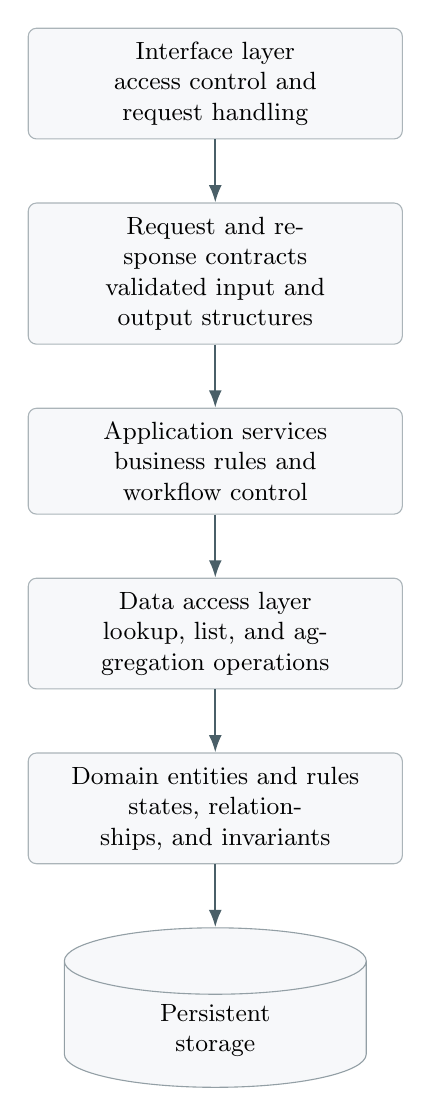
\begin{tikzpicture}[node distance=8mm]
  \node[box, text width=44mm] (interface) {Interface layer\\access control and request handling};
  \node[box, below=of interface, text width=44mm] (contracts) {Request and response contracts\\validated input and output structures};
  \node[box, below=of contracts, text width=44mm] (services) {Application services\\business rules and workflow control};
  \node[box, below=of services, text width=44mm] (dataaccess) {Data access layer\\lookup, list, and aggregation operations};
  \node[box, below=of dataaccess, text width=44mm] (domain) {Domain entities and rules\\states, relationships, and invariants};
  \node[db, below=of domain, text width=36mm] (storage) {Persistent\\storage};

  \draw[arrow] (interface) -- (contracts);
  \draw[arrow] (contracts) -- (services);
  \draw[arrow] (services) -- (dataaccess);
  \draw[arrow] (dataaccess) -- (domain);
  \draw[arrow] (domain) -- (storage);
\end{tikzpicture}%
}
\caption{Component layer stack. Higher layers coordinate interaction, while
lower layers preserve business state and data consistency.}
\end{figure}

\section{Business Rules And State Models}

The domain behavior is organized around explicit state models instead of
implicit status changes hidden inside request handlers.

\begin{table}[!htbp]
\centering
\caption{Core state models}
\begin{tabularx}{\textwidth}{L{0.24\textwidth}L{0.24\textwidth}Y}
\toprule
\textbf{Domain object} & \textbf{Persisted states} & \textbf{Design note} \\
\midrule
Merchant operational status & Pending review, active, rejected, suspended, disabled & Merchant readiness and merchant operating status are related but not identical, so review outcomes and live operating state are tracked separately. \\
\bodyrowrule
Payment transaction & Pending, successful, failed, expired & Payment requests remain pending until confirmed by external evidence or time-based expiration handling. \\
\bodyrowrule
Refund transaction & Refund pending, refunded, refund failed & The system implements full refunds only, and final outcomes depend on external refund evidence. \\
\bodyrowrule
Webhook event & Pending, delivered, failed & Merchant notification delivery is tracked independently from payment and refund finality. \\
\bottomrule
\end{tabularx}
\end{table}

Two design choices are especially important:

\begin{itemize}
  \item payment expiration creates a durable business outcome instead of simply
  removing an old pending request;
  \item ambiguous external evidence produces a reconciliation record instead of
  forcing a risky automatic correction.
\end{itemize}

\section{Asynchronous Event Lifecycle And Recovery}

Although the project does not yet rely on a permanently running background
worker, it already contains the core asynchronous control functions needed for
time-based and retry-based behavior.

\begin{enumerate}
  \item A merchant payment request creates a pending payment with expiration
  metadata.
  \item External payment or refund evidence is stored before the system applies
  state transitions.
  \item Final money-flow outcomes create merchant notification events.
  \item Scheduled processing expires overdue pending payments and continues
  delivery attempts for due notifications.
  \item Delivery failures and ambiguous outcomes are preserved as operational
  evidence rather than being hidden.
  \item Internal users can retry eligible failed notifications without
  changing already-final payment or refund outcomes.
\end{enumerate}

This separation keeps the architecture testable. Core business decisions remain
inside focused application services, while any future scheduling layer can stay
thin and orchestration-oriented.

\chapter{Database Design}

\section{Entity Model}

The data model is designed around durable business evidence. It must support
merchant readiness, transaction state, refund state, notification delivery,
external outcome evidence, reconciliation, audit history, and human account
access without losing traceability.

\begin{landscape}
\begin{figure}[H]
\centering
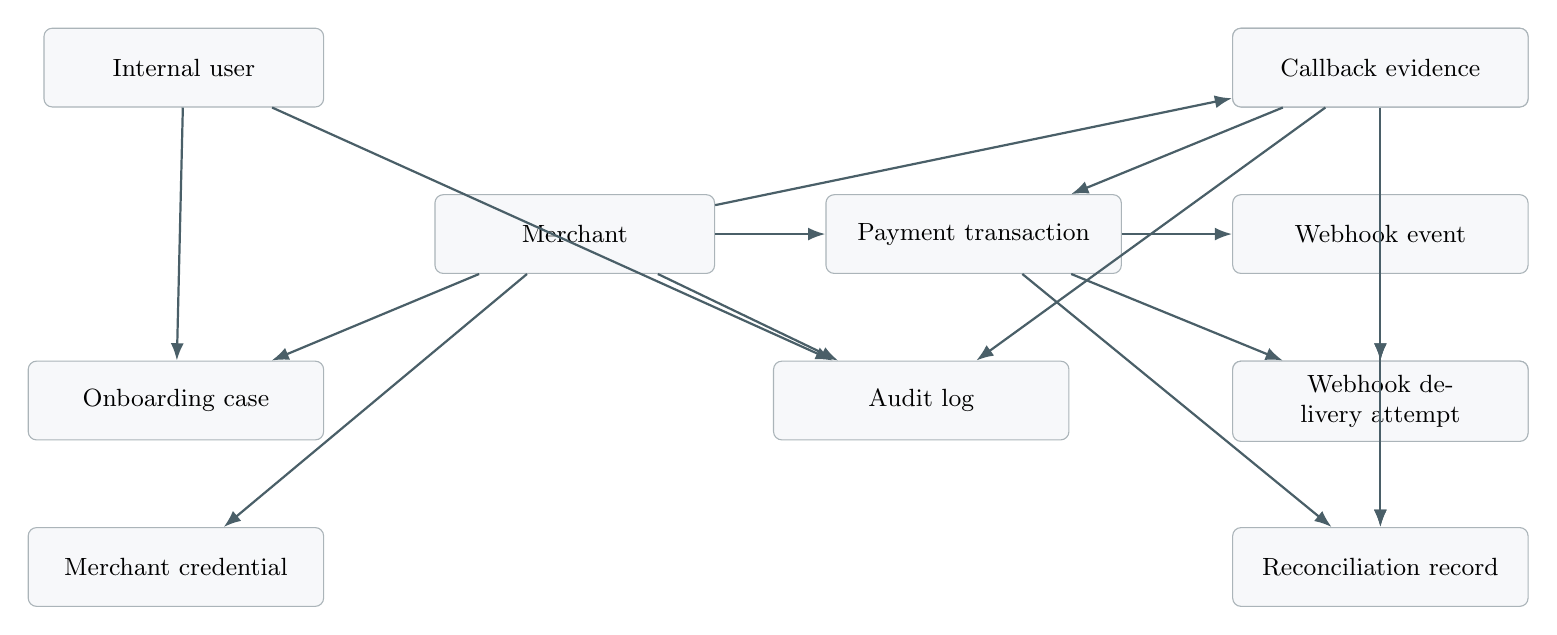
\begin{tikzpicture}[node distance=11mm and 14mm]
  \node[box, text width=32mm] (merchant) {Merchant};
  \node[box, above left=of merchant, text width=32mm] (internalUser) {Internal user};
  \node[box, below left=of merchant, text width=34mm] (onboarding) {Onboarding case};
  \node[box, below=of onboarding, text width=34mm] (credential) {Merchant credential};
  \node[box, right=of merchant, text width=34mm] (payment) {Payment transaction};
  \node[box, above right=of payment, text width=34mm] (merchantUser) {Merchant dashboard user};
  \node[box, below right=of payment, text width=34mm] (refund) {Refund transaction};
  \node[box, right=of payment, text width=34mm] (webhook) {Webhook event};
  \node[box, below=of webhook, text width=34mm] (attempt) {Webhook delivery attempt};
  \node[box, above=of webhook, text width=34mm] (callback) {Callback evidence};
  \node[box, below=of refund, text width=34mm] (recon) {Reconciliation record};
  \node[box, below=of merchant, text width=34mm, xshift=44mm] (audit) {Audit log};

  \draw[arrow] (merchant) -- (onboarding);
  \draw[arrow] (merchant) -- (credential);
  \draw[arrow] (merchant) -- (merchantUser);
  \draw[arrow] (merchant) -- (payment);
  \draw[arrow] (payment) -- (refund);
  \draw[arrow] (payment) -- (webhook);
  \draw[arrow] (webhook) -- (attempt);
  \draw[arrow] (callback) -- (payment);
  \draw[arrow] (callback) -- (refund);
  \draw[arrow] (callback) -- (recon);
  \draw[arrow] (payment) -- (recon);
  \draw[arrow] (refund) -- (recon);
  \draw[arrow] (internalUser) -- (onboarding);
  \draw[arrow] (internalUser) -- (audit);
  \draw[arrow] (merchantUser) -- (audit);
  \draw[arrow] (merchant) -- (audit);
\end{tikzpicture}
\caption{Logical entity relationship overview. The model centers on merchants,
transactions, delivery evidence, and operational traceability.}
\end{figure}
\end{landscape}

\section{Core Entities}

\begin{longtable}{L{0.26\textwidth}L{0.64\textwidth}}
\caption{Core business entities}\\
\toprule
\textbf{Entity} & \textbf{Purpose} \\
\midrule
\endfirsthead
\toprule
\textbf{Entity} & \textbf{Purpose} \\
\midrule
\endhead
Merchant & Stores the merchant identity, operating profile, contact data, notification destination, settlement information, and current operating status. \\
Onboarding Case & Stores merchant-submitted readiness information, review findings, approval or rejection outcomes, and review history. \\
Merchant Credential & Stores merchant integration credential metadata and protected secret material used for signed transaction requests. \\
Merchant Dashboard User & Stores human merchant accounts that sign in to the merchant dashboard and are scoped to one merchant. \\
Internal User & Stores internal administrative and operational accounts used for management and review workflows. \\
Payment Transaction & Stores payment attempts, money amounts, state, expiration information, merchant references, and externally linked payment evidence. \\
Refund Transaction & Stores refund requests and their linkage to successful original payments. \\
Webhook Event & Stores merchant notification payloads, delivery state, retry metadata, and notification history. \\
Webhook Delivery Attempt & Stores individual delivery attempts so the system can preserve delivery evidence over time. \\
Callback Evidence & Stores raw and normalized external outcome evidence for payments and refunds. \\
Reconciliation Record & Stores manual-review evidence when external outcomes do not align cleanly with internal state. \\
Audit Log & Stores durable review and administrative evidence for sensitive human actions. \\
\bottomrule
\end{longtable}

\section{Data Invariants}

\begin{longtable}{L{0.34\textwidth}L{0.56\textwidth}}
\caption{Important data invariants}\\
\toprule
\textbf{Invariant} & \textbf{Reason} \\
\midrule
\endfirsthead
\toprule
\textbf{Invariant} & \textbf{Reason} \\
\midrule
\endhead
Each merchant has one stable public merchant identity. & External integrations and both dashboards need one durable merchant anchor. \\
Only one active merchant integration credential exists at a time. & Signed requests should resolve to one authoritative active credential for each merchant. \\
Each merchant dashboard user belongs to exactly one merchant. & Merchant dashboard access must remain tenant-scoped and must not leak across merchants. \\
Only one active pending payment can exist for the same merchant order at a time. & This prevents duplicate active checkout attempts for one business order. \\
Refund requests are unique per merchant refund reference. & The system needs business-level idempotency for merchant refund initiation. \\
At most one successful full refund can exist for one successful payment. & The project implements full-refund-only behavior. \\
Notification delivery history is preserved separately from notification state. & Final notification status and the evidence that led to it must both remain available. \\
Protected secrets and plaintext passwords are never returned through ordinary read views. & Human access and merchant integration credentials must remain protected even when metadata is viewable. \\
\bottomrule
\end{longtable}

\section{Data Evolution}

The data model evolves by extending business capabilities rather than by
rewriting existing evidence. As the system grows, new entities or attributes
can be introduced for additional merchant lifecycle information, expanded
notification channels, or richer reconciliation support while preserving
historical transaction and audit integrity.

\chapter{User Interface Design}

\section{Two Dashboard Applications}

The project uses two dashboard applications because internal operators and
merchant users have different permissions, risks, and workflows.

\begin{table}[H]
\centering
\caption{Dashboard split}
\begin{tabularx}{\textwidth}{L{0.24\textwidth}L{0.24\textwidth}Y}
\toprule
\textbf{UI} & \textbf{Audience} & \textbf{Purpose} \\
\midrule
Ops Dashboard & Internal Admin/Ops & Operate merchants, investigate evidence, manage users, and recover failed workflows. \\
Merchant Dashboard & Merchant dashboard users & Read merchant-scoped payment, refund, webhook, profile, credential, and analytics data. \\
\bottomrule
\end{tabularx}
\end{table}

This split is not only visual. It mirrors the access model of the system:
internal session cookies and RBAC for Ops, and merchant-scoped portal sessions
for dashboard users. The result is a clearer user experience and stronger data
separation.

\section{Ops Dashboard UI}

The Ops Dashboard is designed for repeated operational work. It favors dense but
readable list and detail layouts, explicit lifecycle actions, semantic badges,
and direct access to operational evidence such as onboarding data, credentials,
payments, refunds, webhook attempts, audit logs, and reconciliation records.

\begin{figure}[H]
\centering
\safeimage{ops-overview.png}{Ops Dashboard overview showing internal metrics and work queues.}
\caption{Ops Dashboard overview. The landing page is optimized for operational
prioritization and queue awareness.}
\end{figure}

\begin{figure}[H]
\centering
\safeimage{ops-merchant-detail.png}{Ops merchant detail with lifecycle status, credential metadata, portal users, onboarding evidence, recent payments, and audit.}
\caption{Ops merchant detail. Merchant status, onboarding evidence, credential
metadata, and portal-user provisioning are grouped into one internal workflow.}
\end{figure}

\section{Merchant Dashboard UI}

The Merchant Dashboard is read-only except for local password change. It gives
merchant users an overview first, then deeper analytics and explorer pages for
support or business questions. Long values such as webhook URLs, QR payloads,
and JSON snippets are wrapped or scrollable to avoid layout overflow.

\begin{figure}[H]
\centering
\begin{subfigure}{0.48\textwidth}
  \centering
  \safeimage[\linewidth]{merchant-overview.png}{Merchant Overview with summary cards and compact charts.}
  \caption{Overview}
\end{subfigure}
\hfill
\begin{subfigure}{0.48\textwidth}
  \centering
  \safeimage[\linewidth]{merchant-analytics.png}{Merchant Analytics with interactive Recharts, tooltips, and data tables.}
  \caption{Analytics}
\end{subfigure}
\caption{Merchant Dashboard overview and analytics.}
\end{figure}

\begin{figure}[H]
\centering
\begin{subfigure}{0.48\textwidth}
  \centering
  \safeimage[\linewidth]{merchant-payments.png}{Merchant payment explorer with filters and detail panel.}
  \caption{Payments}
\end{subfigure}
\hfill
\begin{subfigure}{0.48\textwidth}
  \centering
  \safeimage[\linewidth]{merchant-webhooks.png}{Merchant webhook explorer with event status and attempts.}
  \caption{Webhooks}
\end{subfigure}
\caption{Merchant explorer pages.}
\end{figure}

\begin{figure}[H]
\centering
\begin{subfigure}{0.48\textwidth}
  \centering
  \safeimage[\linewidth]{merchant-profile.png}{Read-only merchant profile and integration metadata.}
  \caption{Profile}
\end{subfigure}
\hfill
\begin{subfigure}{0.48\textwidth}
  \centering
  \safeimage[\linewidth]{merchant-credentials.png}{Credential metadata without raw secret.}
  \caption{Credentials}
\end{subfigure}
\caption{Read-only merchant metadata pages.}
\end{figure}

\section{Responsive And State Design}

Both dashboards treat asynchronous state as a first-class design concern:

\begin{itemize}
  \item loading, error, and empty states are explicit on data-fetching routes;
  \item long tables and side panels remain scrollable instead of forcing layout
  overflow;
  \item chart data is paired with readable labels and tables so exact values are
  not hidden behind hover-only interactions;
  \item session and status panels remain visually stable to reduce user
  confusion during multi-step workflows;
  \item the merchant login form uses explicit labels and accessible field
  associations.
\end{itemize}

\chapter{Component Implementation}

\section{Backend Implementation}

The backend implementation is organized by API surface and business workflow.
Controllers define endpoint paths and dependencies. Services enforce business
rules such as merchant readiness, payment idempotency, refund eligibility,
webhook retry policy, RBAC, audit, and merchant portal scoping. Repositories
hold focused persistence and aggregation queries.

Important implementation points include:

\begin{itemize}
  \item internal auth and merchant portal auth are implemented as separate
  session systems;
  \item merchant-scoped read APIs derive scope from authenticated context rather
  than trusting request parameters;
  \item callback processing and reconciliation are implemented as explicit
  service logic instead of ad hoc controller branches;
  \item write actions that matter operationally emit audit rows with masked
  before and after state snapshots.
\end{itemize}

The Merchant Portal feature introduced a dedicated portal account model,
\texttt{merchant\_users}, and a separate session-auth service. This avoids the
anti-pattern of using HMAC API credentials for human dashboard login. Internal
\texttt{ADMIN} users create and reset merchant portal users from the Ops
Dashboard; generated passwords are returned once and only password hashes are
stored.

\section{Frontend Implementation}

The Ops Dashboard and Merchant Dashboard are separate React, Vite, and
TypeScript applications. Both use React Router for navigation and TanStack
Query for server state. The Merchant Dashboard analytics page uses Recharts for
interactive charts, tooltips, and compact visual summaries.

Important frontend implementation details include:

\begin{itemize}
  \item list and detail layouts for operational scanning on desktop;
  \item responsive one-column behavior on smaller screens;
  \item loading, error, and empty states for async data;
  \item scrollable long lists for recent payments, audit logs, portal users,
  webhooks, credentials, and chart data tables;
  \item stable status and session panels so context does not jump between pages;
  \item explicit label associations on the merchant login form for
  accessibility.
\end{itemize}

\section{Asynchronous Service Implementation}

The current implementation includes the key asynchronous business operations as
callable application services:

\begin{itemize}
  \item payment expiration service for overdue pending payments;
  \item webhook event factory for payment and refund final states;
  \item webhook delivery service with retry scheduling and attempt persistence;
  \item reconciliation services for mismatched or late provider evidence;
  \item internal manual retry endpoint for failed webhook events.
\end{itemize}

However, the project does not yet include a standalone long-running scheduler or
worker runtime as part of the deployed stack. The implemented services are
ready to be invoked by a scheduler or worker trigger, and this boundary is
tested in the backend suite.

\section{Demo Data Implementation}

The demo seed script is explicit and idempotent. It creates a demo merchant,
portal user, credential metadata, payments, refund rows, webhooks, delivery
attempts, and callback evidence. The script does not run automatically on
deploy because production-like deployments should not silently create demo
users.

\begin{lstlisting}[language=bash,caption={Manual demo seed command}]
cd backend
python scripts/seed_dashboard_demo.py
\end{lstlisting}

For sandbox container deployment, the equivalent command is:

\begin{lstlisting}[language=bash,caption={Sandbox demo seed command}]
cd /opt/mini-payment-gateway
docker compose -f docker-compose.sandbox.yml run --rm backend \
  python scripts/seed_dashboard_demo.py
\end{lstlisting}

\chapter{API Design and Implementation}

\section{API Design Strategy}

The API design separates actor responsibilities instead of forcing every actor
through one shared access model. This decision keeps merchant integration,
internal operations, and merchant dashboard access aligned with their real
security and data-visibility needs.

Detailed request and response contracts are maintained in a separate API
reference. This chapter focuses on the boundary design decisions that shape the
overall interface.

\section{API Families And Access Boundaries}

\begin{table}[H]
\centering
\caption{API families and access boundaries}
\begin{tabularx}{\textwidth}{L{0.18\textwidth}L{0.22\textwidth}L{0.22\textwidth}Y}
\toprule
\textbf{API family} & \textbf{Primary actor} & \textbf{Authentication model} & \textbf{Design purpose} \\
\midrule
Internal authentication and administration & Admin or Ops user & Internal session authentication & Supports internal sign-in, account management, and operational access control. \\
Merchant transaction APIs & Merchant backend & Signed merchant integration credentials & Supports payment creation, payment lookup, refund creation, and refund lookup for merchant systems. \\
Provider callback APIs & Provider callback source & Controlled external callback trust model & Accepts external outcome evidence for payments and refunds. \\
Internal operations APIs & Admin or Ops user & Internal session authentication & Supports merchant management, evidence review, reconciliation, notification recovery, and dashboard reads. \\
Merchant dashboard APIs & Merchant dashboard user & Merchant session authentication & Supports merchant-scoped overview, analytics, record exploration, profile views, and credential metadata views. \\
Outbound notification contract & Merchant callback endpoint & Signed gateway-to-merchant notification model & Delivers final payment and refund events to merchant-owned callback destinations. \\
\bottomrule
\end{tabularx}
\end{table}

\section{Authentication Model Split}

The system uses three separate authentication models because the actors carry
three different risk profiles:

\begin{itemize}
  \item merchant backends use signed integration credentials for machine-to-
  machine transaction requests;
  \item internal users use session-based authentication for review and
  administration workflows;
  \item merchant dashboard users use a separate merchant-scoped session model
  for human access to merchant data.
\end{itemize}

This split prevents two common design problems: using human dashboard login for
machine integration, and using merchant integration credentials for interactive
dashboard access.

\section{Asynchronous API And Event Design}

The interface design must safely accept delayed external evidence and delayed
merchant notification delivery. For that reason, provider callbacks and
merchant notifications are treated as durable event flows rather than as simple
status updates.

When external evidence arrives, the system first preserves the evidence and then
applies state rules. If the evidence conflicts with the current internal state,
the system creates a reconciliation path rather than forcing an unsafe
automatic correction.

Merchant notification delivery is also decoupled from transaction finality. A
payment or refund can be final even if merchant notification delivery fails
temporarily. This makes retry and manual recovery possible without rewriting the
underlying money-flow outcome.

\section{Error Model And Data Exposure Rules}

The API design uses stable business error codes so that calling systems and
internal users can distinguish validation failure, readiness failure,
authentication failure, and business-rule conflict.

Sensitive data exposure is minimized throughout the interface design:

\begin{itemize}
  \item raw merchant secrets are not exposed in ordinary read views;
  \item generated one-time passwords are shown only at the moment of creation
  or reset;
  \item merchant dashboard reads remain scoped to the signed-in merchant;
  \item operational evidence is preserved for investigation without exposing
  secret material unnecessarily.
\end{itemize}

\chapter{Testing and Evaluation}

\section{Testing Strategy}

Testing is layered around business risk. Unit and service tests cover isolated
rules such as HMAC verification, merchant readiness, payment idempotency,
refund eligibility, expiration handling, webhook retry policy, and
reconciliation. Route tests cover FastAPI contracts and status codes. End-to-
end tests cover complete business journeys through controllers and services.
Frontend tests cover transforms, rendering, route behavior, type safety, and
build correctness.

\begin{longtable}{L{0.22\textwidth}L{0.34\textwidth}L{0.34\textwidth}}
\caption{Testing and evaluation matrix}\\
\toprule
\textbf{Category} & \textbf{Coverage} & \textbf{Evidence} \\
\midrule
\endfirsthead
\toprule
\textbf{Category} & \textbf{Coverage} & \textbf{Evidence} \\
\midrule
\endhead
Backend unit and service & Auth, readiness, payment, refund, expiration, callback, webhook, reconciliation, audit. & Python \texttt{unittest} suite under \code{backend/tests/}. \\
Backend route & Merchant APIs, provider callbacks, Ops APIs, Merchant Portal APIs, internal auth, internal users. & FastAPI controller and route tests. \\
Backend E2E & Onboarding to payment, refund, webhook, late callback reconciliation, and manual webhook retry. & \code{test_e2e_payment_refund_webhook.py}. \\
Merchant Portal scope & Auth, inactive user rejection, profile and credential secrecy, merchant-specific explorers, analytics ranges and zero buckets. & Merchant portal route and analytics tests. \\
Frontend Merchant Dashboard & Analytics transforms, chart render, route behavior, login accessibility, typecheck, build. & Vitest, TypeScript, and Vite build. \\
Frontend Ops Dashboard & Typecheck and production build. & TypeScript and Vite build. \\
Deployment configuration & Compose syntax and sandbox env requirements. & Docker Compose config validation. \\
Browser smoke & Login, dashboards, list and detail pages, analytics, mobile layout, and overflow checks. & Manual checklist in \code{docs/testing/README.md}. \\
\bottomrule
\end{longtable}

\section{Verification Commands}

\begin{lstlisting}[language=bash,caption={Backend verification}]
cd backend
python -m unittest discover tests -v
python -m unittest tests.test_e2e_payment_refund_webhook -v
\end{lstlisting}

\begin{lstlisting}[language=bash,caption={Frontend and compose verification}]
npm run merchant-dashboard:typecheck
npm run merchant-dashboard:test
npm run merchant-dashboard:build
npm run ops-dashboard:typecheck
npm run ops-dashboard:build
docker compose -f docker-compose.yml config --quiet
docker compose --env-file .env.sandbox.example -f docker-compose.sandbox.yml config --quiet
\end{lstlisting}

Historical pass counts and deploy verification snapshots are maintained in
\code{docs/history/completions/}. The report keeps the verification commands and test
coverage model in the foreground, while exact rollout-specific results stay in
the completion records.

\section{Manual Browser Smoke}

Manual smoke testing validates what automated tests cannot fully express:
layout, readable charts, responsive behavior, and practical operator workflows.
The smoke checklist includes:

\begin{itemize}
  \item Ops login, overview, merchant list and detail, lifecycle action,
  portal-user create or reset or deactivate, payments, refunds, webhooks,
  reconciliation, and audit;
  \item Merchant login, overview, analytics range switching, drill-down links,
  payments, refunds, webhooks, profile, credentials, password change, and
  logout;
  \item UI regressions such as horizontal overflow, clipped badges, unreadable
  charts, unstable status panels, and unreadable data tables.
\end{itemize}

\section{Evaluation Summary}

The current testing approach matches the system's main risks well:

\begin{itemize}
  \item merchant-facing business rules are covered at both service and route
  levels;
  \item asynchronous callback and webhook behavior is validated with focused
  service tests and end-to-end scenarios;
  \item dashboard correctness is supported by frontend build checks, targeted
  tests, and manual browser smoke;
  \item deployment wiring is validated separately through compose checks and
  sandbox deployment verification.
\end{itemize}

The remaining evaluation gap is typical for an MVP: browser smoke and internal
deployment verification still complement the automated suite because layout,
operational readability, and sandbox-specific runtime integration are not fully
captured by unit tests alone.


\appendix
\chapter{Demonstration Storyline}

The recommended demo should follow the implemented system rather than a generic
feature tour. It should show actor boundaries and evidence flow.

\begin{enumerate}
  \item Log in to Ops Dashboard as an internal Admin.
  \item Open merchant detail and show merchant status, onboarding case,
  credential metadata, and portal users.
  \item Create or reset a merchant portal user and explain the one-time
  password rule.
  \item Log in to Merchant Dashboard as that merchant user.
  \item Show Overview and Analytics, then read exact values through tooltips or
  data tables.
  \item Drill down from Analytics into Payments, Refunds, and Webhooks.
  \item Open Profile and Credentials to show read-only merchant metadata and
  masked credential information.
  \item If time remains, return to Ops Dashboard and show audit or
  reconciliation evidence.
\end{enumerate}

\begin{table}[H]
\centering
\caption{Demo route map}
\begin{tabularx}{\textwidth}{L{0.25\textwidth}L{0.27\textwidth}Y}
\toprule
\textbf{Step} & \textbf{Screen or API} & \textbf{What to explain} \\
\midrule
Ops login & \texttt{/login} on port 4173 & Internal session boundary and RBAC. \\
Merchant detail & \texttt{/merchants} & Merchant lifecycle, onboarding, credential metadata, and portal users. \\
Portal provisioning & Merchant detail panel & Admin-only generated password rule. \\
Merchant login & \texttt{/login} on port 4174 & Merchant portal session is separate from HMAC API credentials. \\
Analytics & \texttt{/analytics} & Merchant-scoped revenue, status, refund, and webhook health. \\
Explorers & \texttt{/payments}, \texttt{/refunds}, \texttt{/webhooks} & Drill-down support workflow. \\
Profile or credentials & \texttt{/profile}, \texttt{/credentials} & Read-only metadata and masked secrets. \\
\bottomrule
\end{tabularx}
\end{table}

\chapter{Limitations And Future Work}

The current MVP intentionally excludes several larger payment-platform
features. They should not be presented as implemented:

\begin{itemize}
  \item production settlement and accounting ledger;
  \item disputes and chargeback workflows;
  \item CSV export or BI-grade reporting;
  \item real-time dashboard polling;
  \item multi-provider routing;
  \item partial refunds;
  \item merchant self-service onboarding;
  \item merchant profile editing;
  \item merchant credential rotation from the Merchant Dashboard;
  \item a standalone long-running scheduler or worker runtime.
\end{itemize}

Natural next improvements include:

\begin{itemize}
  \item scheduler or worker runtime for expiration and due-webhook delivery;
  \item CSV export for analytics and explorer data;
  \item custom date ranges for merchant analytics;
  \item stronger provider callback authentication;
  \item broader operational notification and observability features.
\end{itemize}

Each of these should be planned as a separate feature because it changes API
contracts, runtime topology, data retention expectations, or security
boundaries.


\end{document}
